\documentclass[11pt]{article}

% review = anonymous submission with line numbers; preprint = named, with page numbers.
\usepackage[review]{acl}
\usepackage{times}
\usepackage{latexsym}
\usepackage[T1]{fontenc}
\usepackage[utf8]{inputenc}
\usepackage{microtype}
\usepackage{inconsolata}
\usepackage{graphicx}
\usepackage{booktabs}
\usepackage{amsmath}
\usepackage{xcolor}

% Every number in the text that comes from data or results is a macro written by
% analysis/figures.py; rerun it after new results and recompile.
% generated by analysis/figures.py; do not edit
\newcommand{\nAssocGoldText}{1{,}211}
\newcommand{\nAssocGoldStateName}{56}
\newcommand{\nAssocRepeat}{15}
\newcommand{\nRaw}{21{,}853}
\newcommand{\nKept}{21{,}726}
\newcommand{\nDropped}{127}
\newcommand{\nAmbiguous}{10}
\newcommand{\nLeaks}{1{,}974}
\newcommand{\nAnalysis}{19{,}742}
\newcommand{\nDupOptions}{83}
\newcommand{\nDupOnly}{73}
\newcommand{\nAssocState}{1{,}891}
\newcommand{\nAssocStateLeak}{969}
\newcommand{\nAssocLeak}{1{,}267}
\newcommand{\pctEntity}{84.4}
\newcommand{\pctSpan}{68.3}
\newcommand{\nEntities}{1{,}864}
\newcommand{\rhoPageviews}{0.67}
\newcommand{\nPageviews}{826}
\newcommand{\lenSlope}{-4.95}
\newcommand{\lenR}{-0.59}
\newcommand{\nStates}{36}
\newcommand{\SrcCurves}{CPU pilot (2{,}000 sampled questions, original and one permuted option order); to be replaced by the full run}
\newcommand{\SrcDist}{CPU pilot (2{,}000 sampled questions, original and one permuted option order); to be replaced by the full run}
\newcommand{\SrcFreq}{CPU pilot (2{,}000 sampled questions, original and one permuted option order); to be replaced by the full run}
\newcommand{\SrcRel}{CPU pilot (2{,}000 sampled questions, original and one permuted option order); to be replaced by the full run}
\newcommand{\SrcPatch}{pending}
\newcommand{\SrcModels}{CPU pilot (2{,}000 sampled questions, original and one permuted option order); to be replaced by the full run}
\newcommand{\SrcEffects}{CPU pilot (2{,}000 sampled questions, original and one permuted option order); to be replaced by the full run}
\newcommand{\ResultsSource}{CPU pilot (2{,}000 sampled questions, original and one permuted option order); to be replaced by the full run}


% Placeholders that must be filled once the full GPU run is in.
\newcommand{\todoresult}[1]{\textcolor{red}{\textbf{[TODO-RESULT: #1]}}}
\newcommand{\todocite}[1]{\textcolor{red}{\textbf{[TODO-CITE: #1]}}}
\newcommand{\lstar}{\ell^{*}}

\title{When Does the Answer Form? Crystallization Depth of Indian Cultural Knowledge in Language Models}

\author{Anonymous}

\begin{document}
\maketitle

\begin{abstract}
Language models answer many questions about Indian culture correctly, but little is known about where in the network those answers are formed.
We read out every layer of three open models (Llama-3.1-8B, Qwen2.5-7B, Gemma-2-9B) on \nAnalysis{} multiple-choice questions from SANSKRITI and measure the crystallization depth of each correct answer: the relative layer at which the model settles on it.
Early layers of every model prefer one answer letter regardless of content, so we present each question in all four cyclic option orders and average over them, which removes this bias by design.
We then test a preregistered hypothesis: answers about better-documented entities crystallize earlier, controlling for question form and entity length.
\todoresult{one sentence with the main effect per model, or the equivalence result if null.}
\todoresult{one sentence on whether activation patching agrees with the lens depth.}
Code, data-quality notes and all results are released.
\end{abstract}

\section{Introduction}

Benchmarks of cultural knowledge report whether a model answers correctly.
They do not say how the answer is computed, or whether a correct answer about a festival in Bihar is produced the same way as one about a dish from Maharashtra.
Interpretability work on factual recall gives one way to ask this.
Reading the residual stream through the unembedding \citep{nostalgebraist2020logitlens} or through trained per-layer translators \citep{belrose2023tuned} shows the layer at which a model's prediction becomes stable, and causal methods \citep{meng2022locating,geva-etal-2023-dissecting} show which layers carry the information.

We use this to study Indian cultural knowledge with SANSKRITI \citep{maji-etal-2025-sanskriti}, a benchmark of 21{,}853 questions over \nStates{} states and union territories and sixteen cultural attributes.
For each correctly answered question we measure its \emph{crystallization depth}: the relative layer $d = \lstar / L$ at which the correct answer becomes, and remains, the model's choice.
The idea follows \citet{baldock2021difficulty}, who showed that the layer at which an image classifier's prediction settles tracks how hard or atypical an example is.

Our question is whether depth depends on how well documented the entity is.
Language models know less about rare entities \citep{kandpal2023longtail,mallen-etal-2023-trust}, and Indian regional culture is unevenly represented in web text.
If documentation matters beyond accuracy, then among questions a model gets right, answers about rare entities should form later, reflecting a longer computation or a weaker stored association.
If it does not, depth is a property of the model and the question form, and coverage gaps show up only as errors.
Both outcomes are informative for work on cultural representation in models \citep{yu2025cultrace,chelombitko2026cultural}, and we fixed the analysis, the primary metric and the criteria for a null result in advance (\S\ref{sec:prereg}).

Building the measurement exposed two problems that apply to any layer-wise study of multiple-choice answers.
First, in early and middle layers every model we tested ranks one particular answer letter first for nearly all questions.
A naive first-correct-layer metric therefore reports early crystallization exactly for questions whose gold answer happens to sit at that letter.
We remove this by presenting each question in its four cyclic option orders, so that each answer appears once at each letter, and averaging option probabilities by content.
Second, a single first-correct-layer index is noisy: in our pilot its test-retest correlation between two option orders was below 0.3.
We therefore use a continuous depth, the expected layer of the increase in gold probability, and choose between candidate metrics by split-half reliability under a rule written before the full run.

Our contributions are:
(1) a reliable, letter-bias-free measure of crystallization depth for multiple-choice questions, with its reliability reported;
(2) depth profiles for three model families on Indian cultural knowledge;
(3) a preregistered test of the link between entity documentation and depth, with controls for entity length and question type, and a state-level permutation test;
(4) an activation-patching check of whether lens depth matches the layers where the entity information is causally used; and
(5) a data-quality audit of SANSKRITI, including \nLeaks{} questions whose stem reveals the answer.

\todoresult{Final paragraph of the introduction, written after the run. If H1 is supported: state the size of the effect in layers per SD in each model and what it implies. If null: state the equivalence bound that was met and that depth is set by model and question form, not documentation. In either case, one sentence on patching.}

\section{Related Work}

\paragraph{Layer-wise readouts.}
The logit lens decodes intermediate residual states with the model's own final norm and unembedding \citep{nostalgebraist2020logitlens}.
It is biased in early layers, whose representations are not in the basis the unembedding expects; the tuned lens fixes this with an affine translator per layer, trained so that each layer's decoded distribution matches the final one \citep{belrose2023tuned}.
\citet{wendler-etal-2024-llamas} used the logit lens to show that Llama-2 passes through an English-like latent space when translating between other languages.
We use both lenses and report the tuned lens as a secondary readout.

\paragraph{Prediction depth.}
\citet{baldock2021difficulty} defined the prediction depth of an example as the first layer after which a nearest-neighbour probe agrees with the final prediction, and found that it tracks example difficulty, consistency of learning and margin.
Our crystallization depth is the analogue for a language model's multiple-choice answer, read through a lens rather than a probe.

\paragraph{Where facts are recalled.}
Causal tracing locates factual recall in middle-layer MLPs at the last subject token \citep{meng2022locating}.
\citet{geva-etal-2023-dissecting} describe recall as subject enrichment in early and middle layers followed by attribute extraction by attention at the final position.
\citet{zhang2024patching} compare activation-patching choices and recommend logit-difference metrics and same-distribution corruptions (replacing the subject with another real subject) over Gaussian noise.
Our patching follows that advice: we swap the entity for a same-attribute entity from another state and measure normalised logit-difference recovery.

\paragraph{Frequency and knowledge.}
Question-answering accuracy rises with the number of pretraining documents that mention the relevant entities \citep{kandpal2023longtail}, and with entity popularity measured by Wikipedia pageviews \citep{mallen-etal-2023-trust}.
We use both kinds of signal: exact-string counts in an open pretraining corpus, Dolma \citep{soldaini-etal-2024-dolma}, through the infini-gram engine \citep{liu2024infinigram}, and Wikipedia pageviews as a check.
These studies relate frequency to whether the answer is right; we ask whether it relates to where the answer forms when it is right.

\paragraph{Culture inside the model.}
SANSKRITI \citep{maji-etal-2025-sanskriti} evaluates knowledge of Indian culture across states, union territories and cultural attributes; we use it as released.
CulTrace \citep{yu2025cultrace} traces how cultural knowledge is processed inside models.
CultureScope \citep{zhang2025culturescope} probes cultural understanding along a set of cultural dimensions, as a benchmark.
\citet{chelombitko2026cultural} trace mythological knowledge across 18 open models and find that it is represented in internal layers even when it is not decoded at the output.
We add a frequency-controlled, layer-resolved measure for a single, large regional benchmark.

\section{Method}
\label{sec:method}

\subsection{Data}
\label{sec:data}

We use SANSKRITI \citep{maji-etal-2025-sanskriti} from the Hugging Face Hub (\texttt{13ari/Sanskriti}, fixed revision), \nRaw{} four-option questions about \nStates{} Indian states and union territories, sixteen cultural attributes and four question types (association, state prediction, country prediction, general awareness).
We drop the \nDropped{} rows whose answer field matches none of the options and exclude \nAmbiguous{} rows whose gold text appears in two options.
We also exclude the \nLeaks{} rows whose stem reveals the answer: the stem contains the gold option text, the gold state's name or one of its name forms, demonyms or languages, or ``Indian'' when the gold is India.
This leaves \nAnalysis{} questions (Table~\ref{tab:data}; details in Appendix~\ref{app:data}).

Each question is formatted as
\texttt{Question: \{stem\} A. \{o$_1$\} B. \{o$_2$\} C. \{o$_3$\} D. \{o$_4$\} Answer:}
with each option on its own line, and the model's choice is read at the final token over the four tokens ``\,A'' to ``\,D'' (a leading space; one token in every tokenizer we use).
Every question is run in five option orders: the four cyclic rotations that place the gold answer at A, B, C and D once each, and one seeded random permutation used only for robustness.

\subsection{Models and readouts}

We study the base (not instruction-tuned) Llama-3.1-8B \citep{grattafiori2024llama3}, Qwen2.5-7B \citep{qwen2025qwen25} and Gemma-2-9B \citep{gemma2024gemma2}, with $L = 32$, 28 and 42 blocks, in bfloat16, using Hugging Face \texttt{transformers} with forward hooks.
For readout layer $\ell \in \{0, \dots, L\}$ we take the residual stream at the final prompt token: $\ell = 0$ is the embedding output as it enters the first block (including Gemma's $\sqrt{d}$ scaling) and $\ell \geq 1$ is the output of block $\ell$.

\paragraph{Logit lens.}
We apply the model's final normalisation and unembedding to the layer-$\ell$ state (and Gemma-2's final logit soft-capping) and take a softmax restricted to the four option tokens, giving $p_\ell \in \Delta^3$.
We check that at $\ell = L$ this reproduces the model's own output logits.

\paragraph{Tuned lens.}
Following \citet{belrose2023tuned}, each layer gets an affine translator $T_\ell(h) = h + A_\ell (h / s_\ell) + b_\ell$, initialised to the identity, trained to minimise the KL divergence from the model's final next-token distribution on WikiText-103 \citep{merity2016pointer} text (4M training tokens, SGD with Nesterov momentum).
Here $s_\ell$ is a fixed per-layer scale, the mean Euclidean norm of the layer's residual states on a calibration batch.
Without it, residual norms that grow by two orders of magnitude across layers made a shared learning rate diverge at late layers.
The final layer keeps the identity, so both lenses agree at $\ell = L$.

\subsection{Crystallization depth}

\paragraph{Letter bias.}
In early and middle layers the logit lens ranks one letter first for almost every question (Figure~\ref{fig:curves}, dotted grey lines).
In the pilot, every Llama question whose naive first-correct layer was early had gold answer B, and every such Qwen question had gold A.
A metric defined on one option order therefore measures the letter of the answer as much as the answer.
The four cyclic rotations solve this by design: averaged over them, each option content appears at each letter once, so a letter preference adds the same amount to every option.

\paragraph{Metrics.}
For question $q$ and rotation $r$, let $p^{(r)}_\ell(c)$ be the probability of option content $c$ at layer $\ell$, and let $\bar p_\ell(c)$ be its mean over the four rotations.
We define the following depths, all in layers and divided by $L$ to give $d$:
\begin{itemize}
\itemsep0em
\item $d_{\mathrm{soft}}$: the expected layer under the normalised positive increments of the gold probability, $\sum_\ell \ell\, w_\ell$ with $w_\ell \propto \max(0, \bar p_\ell(g) - \bar p_{\ell-1}(g))$. It is continuous and robust to one-layer flips.
\item $\lstar_{\mathrm{cyc}}$: the first layer at which the gold content has the largest $\bar p_\ell$ and keeps it through $L$.
\item $d_{\mathrm{margin}}$: the first layer after which the rotation-mean of the letter-calibrated gold-minus-best-distractor log-probability margin stays positive. Calibration subtracts each letter's mean log-probability at that layer, estimated over all four rotations together so that gold letters are balanced.
\item $\lstar_{\mathrm{mean}}$ and $\lstar_{\mathrm{cal,mean}}$: the original first-top-1-and-stays layer of each rotation, without and with calibration, averaged over rotations.
\end{itemize}
We analyse questions answered correctly under $\bar p_L$.

\paragraph{Primary metric.}
\label{sec:prereg}
The analysis plan was registered in the repository before the full run (commit \texttt{c05260c}).
$d_{\mathrm{soft}}$ is primary unless one of $\lstar_{\mathrm{cyc}}$ or $d_{\mathrm{margin}}$ is clearly more reliable: in at least two of three models its split-half reliability (rotations $\{0,2\}$ against $\{1,3\}$, Spearman over questions, Spearman--Brown corrected to four rotations) must exceed $d_{\mathrm{soft}}$'s by at least 0.10, with non-overlapping 95\% bootstrap intervals.
\todoresult{name the metric selected by the rule and its reliabilities (results/primary\_metric.json).}

\subsection{Entity documentation}

An entity is extracted from each stem with templates for the templated question forms and a set of patterns for free-form stems (\pctEntity\% of analysed questions have an entity; Appendix~\ref{app:data}).
Its frequency is the exact-string count in Dolma v1.7 through the infini-gram API (index \texttt{v4\_dolma-v1\_7\_llama}), used as $\log(1 + \text{count})$.
Long names are rarer as exact strings: log count falls with log token length (slope \lenSlope, $r = \lenR$ over \nEntities{} entities).
We therefore control for token length and word count, and also report a length-adjusted frequency, the residual of log count on log token length.
As a check on the measure, corpus counts and 2024 English Wikipedia pageviews correlate at Spearman $\rho = \rhoPageviews$ over the \nPageviews{} entities with an article.
State frequency is the log count of the state's name.

\subsection{Statistical analysis}

For each model and depth metric we fit
\begin{multline*}
d \sim z(\text{entity freq}) + z(\text{state freq}) + \text{acc} \\
+ z(\text{stem words}) + z(\log \text{entity tokens}) \\
+ z(\text{entity words}) + \text{attribute} + \text{question type},
\end{multline*}
where acc is the share of the four rotations answered correctly.
The registered estimator is a linear mixed model with a random intercept per state; when its random-effect variance is estimated at the boundary, OLS with standard errors clustered by state is reported instead (both are saved).
The entity-frequency test (H1) is two-sided with Holm correction across the five depth metrics within each model \todocite{Holm 1979}.
The state-frequency test (H2) is a permutation test that shuffles state frequencies across states (1{,}000 permutations).
A result is positive if the primary metric's Holm-adjusted $p < 0.05$ with a negative coefficient in at least two of three models, and null if in at least two models the 90\% interval of the standardised coefficient lies within $\pm 0.10$ depth standard deviations per standard deviation of frequency.

\subsection{Activation patching}

To test whether lens depth matches the layers where the entity is used, we patch the residual stream, in the original option order, on a stratified sample of 1{,}200 questions (frequency tier by attribute, across all eligible states, with Maharashtra and Bihar guaranteed at least 40 each).
The corrupted prompt replaces the entity span with an entity of the same attribute from a different state.
For each layer we copy the clean final-token residual into the corrupted run and measure recovery, $(\mathrm{LD}_{\mathrm{patch}} - \mathrm{LD}_{\mathrm{corr}}) / (\mathrm{LD}_{\mathrm{clean}} - \mathrm{LD}_{\mathrm{corr}})$, where LD is the gold-minus-best-distractor logit difference \citep{zhang2024patching}.
A row is valid if the clean answer is correct and the corruption moves LD by at least one logit.
Patching depth is the first layer with recovery $\geq 0.5$ (0.3 and 0.7 as sensitivity checks), and H3 is its Spearman correlation with $d_{\mathrm{soft}}$.

\section{Results}
\label{sec:results}

All tables and figures in this section are generated by \texttt{analysis/figures.py} from the files in \texttt{results/}.
At the time of writing they show the \ResultsSource{}; captions name the source of each item.
The Gemma pilot stopped at 1{,}536 questions in the original order only, so Gemma appears in Figure~\ref{fig:curves} but not yet in the depth tables.

\begin{table}[t]
\centering\small\setlength{\tabcolsep}{4pt}
\begin{tabular}{lrrrrr}
\toprule
Model & $L$ & $n$ & Acc. & $d_{\mathrm{soft}}$ & $\ell^*_{\mathrm{cyc}}/L$ \\
\midrule
Llama-3.1-8B & 32 & 2{,}000 & 0.831 & 0.49 & 0.56 \\
Qwen2.5-7B & 28 & 2{,}000 & 0.810 & 0.62 & 0.79 \\
Gemma-2-9B & -- & -- & -- & -- & -- \\
\bottomrule
\end{tabular}

\caption{Accuracy (gold content top-1 at layer $L$) and median relative depth of correctly answered questions. Source: \SrcModels{}.}
\label{tab:models}
\end{table}

\begin{figure*}[t]
\centering
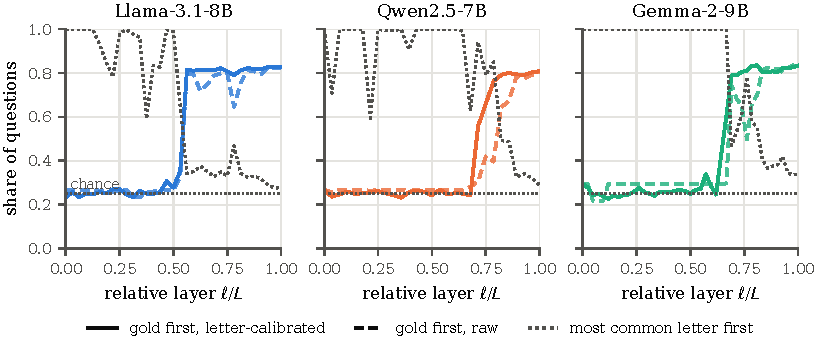
\includegraphics[width=\textwidth]{figures/layer_curves.pdf}
\caption{Logit lens, by relative layer. Coloured lines: share of questions whose gold answer is ranked first, from the raw restricted softmax (dashed) and after subtracting each letter's mean log-probability at that layer (solid). Grey dotted: share of questions on which the single most common letter is ranked first. The black dotted line is chance. Source: \SrcCurves{}.}
\label{fig:curves}
\end{figure*}

\subsection{Where answers crystallize}

Figure~\ref{fig:curves} shows the letter bias and the transition.
Until about half of the depth in Llama and about two thirds in Qwen and Gemma, one letter is ranked first on most questions and the gold answer is ranked first at chance rate.
The share of correct rankings then rises within a few layers to near its final value.
Removing the letter prior makes little difference before this transition and moves the rise slightly earlier, mainly in Qwen; it matters most for per-question depths, where a question whose gold sits at the favoured letter would otherwise be counted as correct from the first layer.
Table~\ref{tab:models} and Figure~\ref{fig:depth} give the depth of correct answers.
\todoresult{Describe the depth distributions per model from the full run: medians of $d_{\mathrm{soft}}$, whether the three models differ in relative depth, and how tuned-lens depths compare to logit-lens depths (tuned lens expected earlier).}

\begin{figure}[t]
\centering
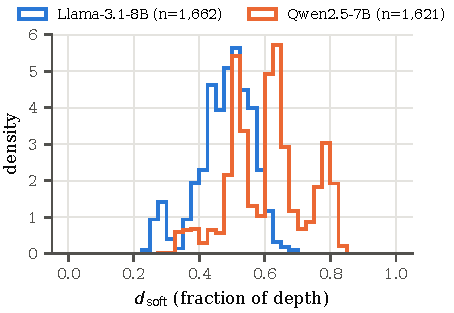
\includegraphics[width=\columnwidth]{figures/depth_distribution.pdf}
\caption{Distribution of $d_{\mathrm{soft}}$ over correctly answered questions. Source: \SrcDist{}.}
\label{fig:depth}
\end{figure}

\subsection{Reliability and choice of metric}

\begin{figure}[t]
\centering
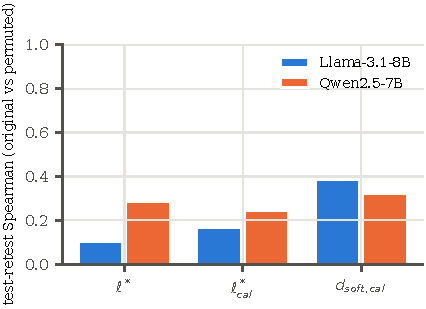
\includegraphics[width=\columnwidth]{figures/reliability.pdf}
\caption{Reliability of the depth metrics on questions correct in both halves or orders. Source: \SrcRel{}.}
\label{fig:reliability}
\end{figure}

Figure~\ref{fig:reliability} reports reliability per metric.
In the pilot, single-order first-correct-layer metrics had test-retest Spearman correlations between 0.10 and 0.28 across the two option orders, and the continuous calibrated depth between 0.32 and 0.39.
\todoresult{split-half reliabilities from the full run for all five metrics and three models, and the outcome of the preregistered rule.}

\subsection{Depth and entity documentation}

\begin{table*}[t]
\centering\small
\begin{tabular}{lccccr}
\toprule
Model & Entity freq. & Holm $p$ & State freq. & Perm.\ $p$ & $n$ \\
\midrule
Llama-3.1-8B & -0.24 [-0.42{,} -0.06] & 0.028 & -0.05 [-0.21{,} +0.11] & 0.58 & 1{,}401 \\
Qwen2.5-7B & +0.18 [-0.07{,} +0.44] & 0.816 & -0.03 [-0.17{,} +0.11] & 0.71 & 1{,}342 \\
Gemma-2-9B & \multicolumn{5}{c}{--} \\
\bottomrule
\end{tabular}

\caption{Effect of one standard deviation of entity frequency (raw log count) and of state frequency on the primary depth metric, in layers, with 95\% confidence intervals (OLS, standard errors clustered by state, all controls). Holm $p$ is adjusted across the five depth metrics. Perm.\ $p$ is the state-label permutation test for state frequency. Source: \SrcEffects{}.}
\label{tab:effects}
\end{table*}

\begin{figure}[t]
\centering
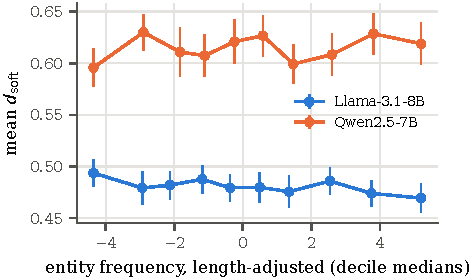
\includegraphics[width=\columnwidth]{figures/frequency.pdf}
\caption{Mean $d_{\mathrm{soft}}$ by decile of length-adjusted entity frequency, with 95\% intervals. Uncontrolled; the tests in Table~\ref{tab:effects} include all controls. Source: \SrcFreq{}.}
\label{fig:freq}
\end{figure}

Table~\ref{tab:effects} and Figure~\ref{fig:freq} report H1 and H2.
In the pilot, which is exploratory and not part of the preregistered test, the entity effect had opposite signs in the two models it covered, and state frequency had no detectable effect.
\todoresult{H1 outcome per the preregistered criteria (positive, null with the equivalence bound, opposite, or inconclusive), with the effect per model in layers per SD; the length-adjusted and pageviews robustness checks; the tuned-lens readout.}
\todoresult{H2 outcome from the permutation test; per-state medians for Maharashtra and Bihar and the extremes.}

\subsection{Activation patching}

\begin{figure}[t]
\centering
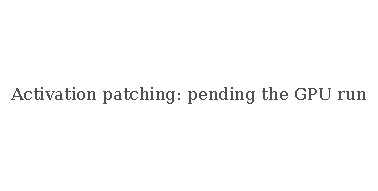
\includegraphics[width=\columnwidth]{figures/patching.pdf}
\caption{Median recovery of the clean logit difference when the clean final-token residual is patched in at each relative layer. Source: \SrcPatch{}.}
\label{fig:patch}
\end{figure}

\todoresult{Number of valid patched questions per model; the layer at which median recovery crosses 0.5; H3 Spearman correlation between patching depth and $d_{\mathrm{soft}}$ with its interval; sensitivity at thresholds 0.3 and 0.7.}

\section{Discussion}

\paragraph{Measuring depth on multiple-choice answers.}
The letter bias in Figure~\ref{fig:curves} is large enough that any layer-wise analysis of multiple-choice answers on a single option order mostly measures where the answer letter is.
Balancing gold positions with cyclic rotations and averaging by content removes it without a learned correction.
Single-layer crystallization indices were also too noisy to support question-level analysis in our pilot, so we recommend continuous depths and reporting their reliability.

\paragraph{What depth tells us about cultural knowledge.}
\todoresult{If H1 positive: better-documented entities resolve earlier; discuss size relative to between-model and between-attribute differences, and what it means for regional coverage. If null: depth is set by model and question form; documentation affects whether, not where, the answer forms; relate to \citet{kandpal2023longtail} and \citet{mallen-etal-2023-trust}. If opposite or mixed: report the models separately and avoid a general claim.}

\paragraph{Lens and causal depth.}
\todoresult{Agreement or disagreement between patching depth and lens depth (H3), and whether the entity information is used before the answer becomes readable.}

\section*{Limitations}

Exact-string counts in one open corpus are a proxy for how often a model saw an entity; the models we study were trained on other, undisclosed data.
Counts depend on spelling and transliteration, which vary widely for Indian names, and our entity extraction misses some entities and fails to find a span in others.
Depth is defined on a multiple-choice format with a fixed prompt, and it is measured only where the model is correct, so it describes a selected subset.
Lenses read out what is linearly decodable through the unembedding or a learned translator; information can be present earlier in a form neither lens decodes.
Patching swaps one entity for another of the same attribute, which also changes token length and familiarity.
We study three base models of 7 to 9 billion parameters.


\bibliography{references}

\appendix
\section{Data Quality}
\label{app:data}

We use SANSKRITI as released and do not change any question.
The full notes, with every affected row, are in \texttt{data/processed/data\_quality.md} and \texttt{leaks.csv} in our repository.

\begin{table}[h]
\centering\small
\begin{tabular}{lr}
\toprule
Rows & Count \\
\midrule
Rows in the release & 21{,}853 \\
Answer matches no option (dropped) & 127 \\
Gold text in two options (excluded) & 10 \\
Stem reveals the answer (excluded) & 1{,}974 \\
Analysis set & 19{,}742 \\
Duplicated distractor (kept, flagged) & 73 \\
\bottomrule
\end{tabular}

\caption{From the release to the analysis set.}
\label{tab:data}
\end{table}

\paragraph{Answer matches no option.}
In \nDropped{} rows the answer field matches none of the four options after trimming and lowercasing.
In most of them the answer field holds the subject of the question or a paraphrase of it rather than an option (for example, the answer to ``What is the primary ingredient used in preparing Dhuska?'' is ``Primary ingredient in Dhuska''), and a few differ by spelling (``Uttarakhand'' against option ``Uttrakhand'').
We drop these rows rather than guess the intended answer.

\paragraph{Ambiguous gold.}
In \nAmbiguous{} rows the gold text appears as two options, so either letter is correct; these are excluded.
A further \nDupOnly{} rows repeat a distractor (two identical wrong options); they are kept and flagged, since the gold answer is unique.

\paragraph{Stems that reveal the answer.}
In \nLeaks{} rows the stem contains the gold option, or a name form or demonym of the gold state (or ``Indian'' when the gold is India).
Most are Association questions: in \nAssocGoldText{} of them the gold text itself appears in the stem, and in \nAssocGoldStateName{} more a name form of the gold state does.
These questions test reading rather than knowledge, so they are excluded from the depth analysis; they remain in the released tables with the flag \texttt{leaks\_answer}.

\paragraph{Association questions answered by the state.}
Association questions ask which region an item belongs to, and their distractors are districts, towns or valleys.
In \nAssocState{} of them the gold option is instead the name of the row's own state, so the question can be answered at state level.
When the templated stem also names the state, as in ``Where is the National Zoological Park famous within Delhi?'' with gold ``Delhi'', the answer is given away; this is the case for \nAssocStateLeak{} of the \nAssocState{} rows, which are among the leaks above.
Because each templated item appears under all three Association templates, the issue sits with those items' answer fields rather than with the templates.
In \nAssocRepeat{} further Association rows the gold option repeats the item named in the stem.

\section{Implementation and Reproduction}
\label{app:impl}

All code is in the repository: \texttt{data/prep.py} (prompts, option orders, leak flags), \texttt{data/entities.py} and \texttt{data/frequency.py} (entities and counts), \texttt{run/forward.py} (residual capture), \texttt{run/tune\_lens.py}, \texttt{analysis/depth.py} (metrics, aggregation, reliability, the primary-metric rule), \texttt{analysis/stats.py} (regressions, Holm, permutation, equivalence), \texttt{run/patch.py} and \texttt{analysis/figures.py}.
The seed is 1234 throughout.
The random permutation order of each question is derived from the seed and the question id, so it is the same on every machine.
The analysis plan, \texttt{ANALYSIS\_PLAN.md}, was registered before the full run; any deviation is appended to it with a date and a reason.
\todoresult{GPU type, run time per model and package versions from the results archive.}


\end{document}
